\chapter{Hoe dieren zich voortplanten}\label{ch:g4:animal-reproduction}

In mei staat de vijver vol kikkergezang; in juni is hij zwart van de
\omterm{ex:g2:animals-grow-up:frog}{donderpadden}. Het gezang bleek het begin van het verhaal te zijn: de
voortplanting --- hoe \omterm{def:g1:animals-around-us:animal}{dieren} de volgende generatie maken --- volgt
regels die van kikkers tot olifanten gelden, met prachtige variaties in
de details.

\section{Er zijn er twee voor nodig}

\begin{definition}[Geslachtelijke voortplanting]\label{def:g4:animal-reproduction:sexual}
Bij \omterm{def:g1:animals-around-us:animal}{dieren} zijn er om jongen te maken meestal twee ouders nodig: een
\emph{vrouwtje}\index{vrouwtje} en een \emph{mannetje}\index{mannetje}.
Het vrouwtje maakt \emph{eicellen}\index{eicel}; het mannetje maakt
\emph{zaadcellen}\index{zaadcel}. Een jong \omterm{def:g1:animals-around-us:animal}{dier} begint wanneer één
zaadcel zich met één eicel verenigt --- dat samengaan heet
\emph{bevruchting}\index{bevruchting}. Voortplanting met twee ouders
heet \emph{geslachtelijke voortplanting}\index{geslachtelijke voortplanting}.
\end{definition}

\begin{example}[Waarom de kikkers zingen]\label{ex:g4:animal-reproduction:song}
Het koor van mei zijn de \omterm{def:g4:animal-reproduction:sexual}{mannetjes} die de \omterm{def:g4:animal-reproduction:sexual}{vrouwtjes} naar de vijver
roepen. Elk paar laat daarna zijn cellen in het water los --- de
eitjes van het \omterm{def:g4:animal-reproduction:sexual}{vrouwtje}, het \omterm{def:g2:from-seed-to-plant:seed}{zaad} van het \omterm{def:g4:animal-reproduction:sexual}{mannetje} --- en daar vindt de
\omterm{def:g4:animal-reproduction:sexual}{bevruchting} plaats. De zwarte stipjes in de gelei zijn een paar dagen
later de jongen die al groeien: het gezang was stap één van de
kikkercyclus uit \cref{ch:g2:animals-grow-up}.
\end{example}

\begin{omfigure}
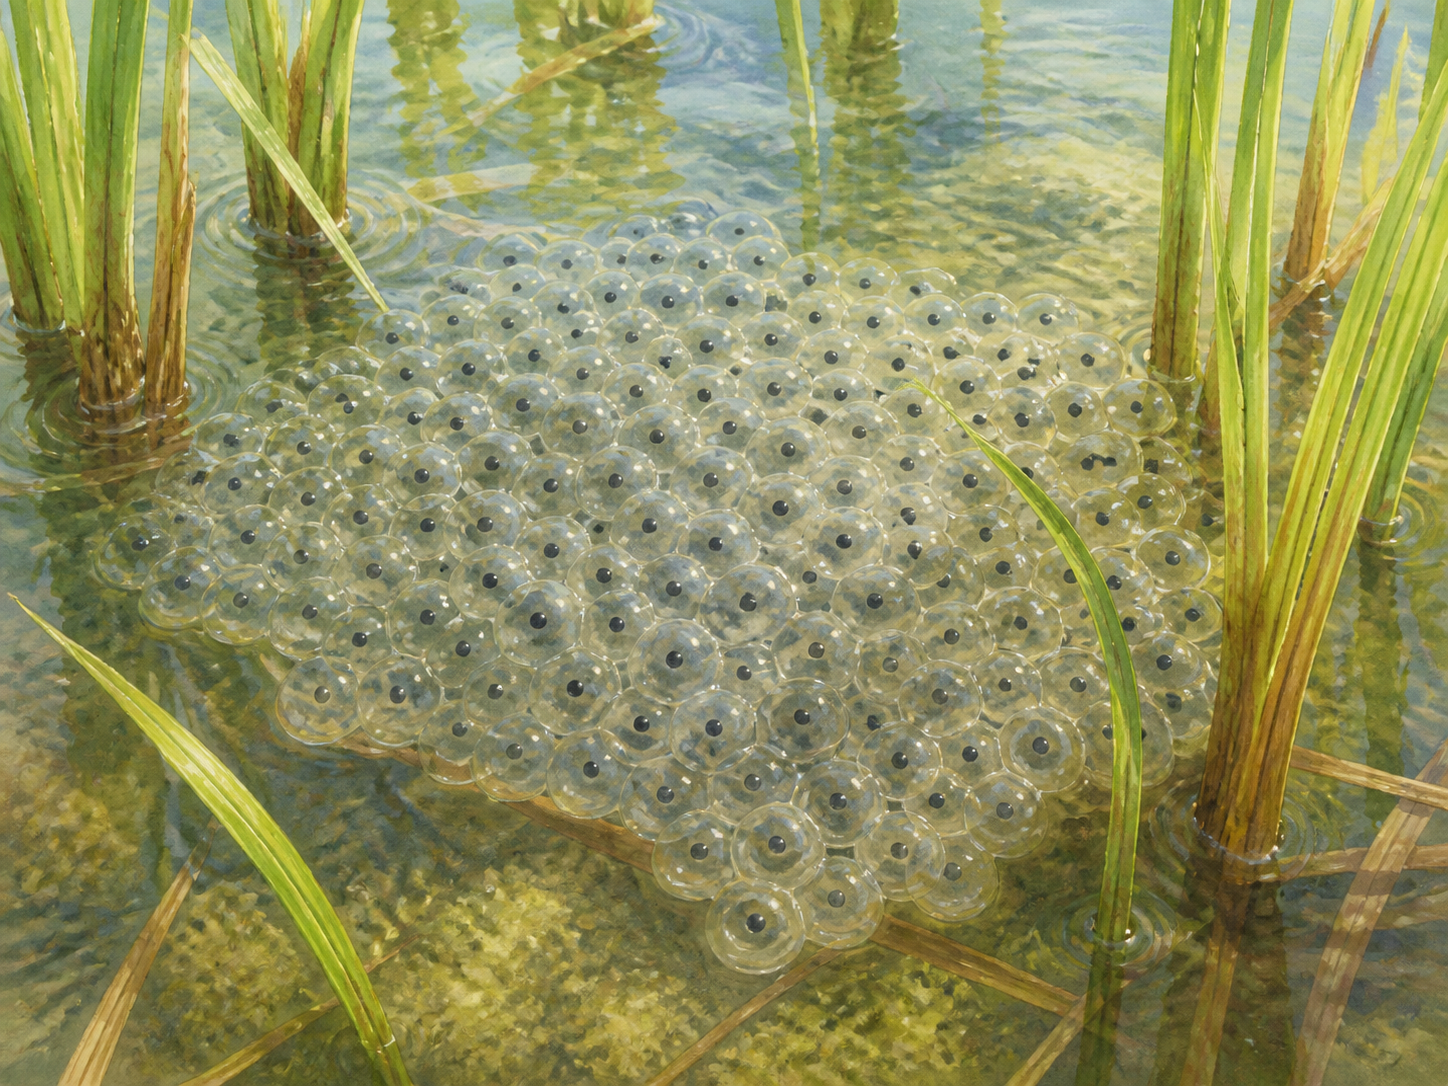
\includegraphics[width=0.56\linewidth]{images/book1/ai/g4-repro-frogspawn.png}

{\small Een paar dagen na het koor: kikkerdril tussen het riet, elk
geleibolletje een bevrucht eitje met daarin het begin van een jonge kikker.}
\end{omfigure}

\begin{remark}[Twee ouders, gemengd geluk]\label{rem:g4:animal-reproduction:mix}
Een jong \omterm{def:g1:animals-around-us:animal}{dier} krijgt van elke ouder iets mee --- en daarom kan een
veulen de kleur van zijn moeder en de witte bles van zijn vader hebben.
Wat elke ouder precies doorgeeft, en hoe, is een van de grote vragen
verderop in dit boek; onthoud voorlopig alleen dat elk geslachtelijk
verwekt \omterm{def:g1:animals-around-us:animal}{dier} twee ouders heeft en op allebei lijkt.
\end{remark}

\section{Eieren gelegd, of jongen levend geboren}

\begin{definition}[Eierleggend en levendbarend]\label{def:g4:animal-reproduction:ovivivi}
De twee manieren van \omterm{def:g2:born-grow-die:cycle}{geboren} worden uit
\cref{def:g2:animals-grow-up:born} krijgen nu hun wetenschappelijke namen:
\begin{itemize}
  \item een \omterm{def:g1:animals-around-us:animal}{dier} is \emph{eierleggend}\index{eierleggend} als het
        \omterm{def:g4:animal-reproduction:sexual}{vrouwtje} \emph{eieren} legt en de jongen buiten haar lichaam,
        in het \omterm{def:g2:animals-grow-up:born}{ei}, uitgroeien: \omterm{prop:g3:sorting-living-things:groups}{vogels}, de meeste \omterm{prop:g3:sorting-living-things:groups}{vissen}, de meeste
        \omterm{prop:g4:classifying-animals:classes}{reptielen}, \omterm{prop:g3:sorting-living-things:groups}{amfibieën}, \omterm{prop:g3:sorting-living-things:groups}{insecten}, slakken;
  \item een \omterm{def:g1:animals-around-us:animal}{dier} is \emph{levendbarend}\index{levendbarend} als het jong
        \emph{in het lichaam van de moeder} groeit, door haar gevoed
        wordt, en \emph{\omterm{def:g2:animals-grow-up:born}{levend geboren}} wordt: bijna alle \omterm{prop:g3:sorting-living-things:groups}{zoogdieren}.
\end{itemize}
\end{definition}

\begin{example}[Twee kraamkamers]\label{ex:g4:animal-reproduction:nurseries}
Het kuiken van de kip brengt drie warme weken door in een \omterm{def:g2:animals-grow-up:born}{ei} met schaal
en leeft van de dooier (\cref{rem:g2:animals-grow-up:egg}); het veulen
brengt elf maanden door in de merrie, doorlopend gevoed door haar
lichaam, en wordt \omterm{def:g2:born-grow-die:cycle}{geboren} en staat binnen het uur op zijn poten.
Hetzelfde doel, twee kraamkamers: het ene een lunchpakket in een schaal,
het andere roomservice vanbinnen.
\end{example}

\begin{proposition}[Waar de bevruchting plaatsvindt]\label{prop:g4:animal-reproduction:where}
Bij waterbewoners als \omterm{prop:g3:sorting-living-things:groups}{vissen} en kikkers vindt de \omterm{def:g4:animal-reproduction:sexual}{bevruchting} meestal
\emph{in het water} plaats, buiten het lichaam van het \omterm{def:g4:animal-reproduction:sexual}{vrouwtje} ---
eitjes en \omterm{def:g2:from-seed-to-plant:seed}{zaad} worden samen losgelaten en ontmoeten elkaar bij
duizenden. Bij landdieren --- \omterm{prop:g3:sorting-living-things:groups}{vogels}, \omterm{prop:g4:classifying-animals:classes}{reptielen}, \omterm{prop:g3:sorting-living-things:groups}{zoogdieren}, \omterm{prop:g3:sorting-living-things:groups}{insecten}
--- zouden de cellen in de open lucht uitdrogen, dus brengt het
\omterm{def:g4:animal-reproduction:sexual}{mannetje} zijn \omterm{def:g2:from-seed-to-plant:seed}{zaad} \emph{in het lichaam van het \omterm{def:g4:animal-reproduction:sexual}{vrouwtje}} tijdens de
\emph{paring}\index{paring}, en daar vindt de \omterm{def:g4:animal-reproduction:sexual}{bevruchting} plaats.
\end{proposition}
\admitted

\section{Weinig jongen en veel zorg, of veel jongen en geen}

\begin{proposition}[Twee strategieën voor de volgende generatie]\label{prop:g4:animal-reproduction:strategies}
Vergelijk de aantallen: een kabeljauw laat \emph{miljoenen} eitjes per
jaar los en zorgt voor geen enkel; een olifant krijgt om de paar jaar
\emph{één} kalf en bewaakt het tien jaar lang. Tussen die uitersten
geldt een regel in de hele dierenwereld: hoe meer jongen een soort
maakt, hoe minder zorg elk krijgt --- en hoe minder ze er maakt, hoe
meer elk beschermd en gevoed wordt. Beide strategieën slagen: gemiddeld
overleven er genoeg jongen om de ouders te vervangen.
\end{proposition}
\admitted

\begin{example}[De vijver tellen]\label{ex:g4:animal-reproduction:pondcount}
Het legsel van één kikkerpaar bevat duizenden eitjes. Reigers,
stekelbaarzen en libellenlarven (zie \cref{ex:g3:food-chains:three})
eten het hele voorjaar \omterm{ex:g2:animals-grow-up:frog}{donderpadden} --- en van die duizenden klimmen er
in juli een handvol kikkertjes de oever op. Het enorme legsel is geen
verspilling: het is het antwoord van de kikker op de gevaren van de
vijver, helemaal zonder ouderlijke bewaking.
\end{example}

\begin{example}[Het andere uiterste]\label{ex:g4:animal-reproduction:whalecalf}
Het walviskalf wordt alleen \omterm{def:g2:born-grow-die:cycle}{geboren}, zwemt meteen naast zijn moeder,
drinkt maandenlang haar rijke \omterm{def:g2:animals-grow-up:born}{melk} en wordt tegen elk gevaar verdedigd.
Eén jong tegelijk --- maar dat ene krijgt alles. \omterm{prop:g3:sorting-living-things:groups}{Zoogdieren}, met hun
\omterm{def:g2:animals-grow-up:born}{melk} (\cref{def:g2:animals-grow-up:born}), zijn de grote specialisten
van de strategie van weinig-en-goed-verzorgd.
\end{example}

\begin{method}[De strategie van een soort aflezen]\label{met:g4:animal-reproduction:read}
Vraag je bij een soort af:
\begin{enumerate}
  \item Hoeveel jongen tegelijk --- één, een stuk of tien, duizenden?
  \item Wie bewaakt en voedt ze --- beide ouders, de moeder, niemand?
  \item Waar beginnen ze --- in een \omterm{def:g2:animals-grow-up:born}{ei} buiten, of gegroeid vanbinnen?
  \item Controleer het evenwicht van
        \cref{prop:g4:animal-reproduction:strategies}: veel jongen met
        weinig zorg, of weinig met veel.
\end{enumerate}
\end{method}

\section{Oefeningen}

\begin{exercise}[$\star$]\label{exo:g4:animal-reproduction:1}
Wat is \omterm{def:g4:animal-reproduction:sexual}{bevruchting}? Welke cel komt van welke ouder?
\end{exercise}

\begin{exercise}[$\star$]\label{exo:g4:animal-reproduction:2}
Omschrijf \omterm{def:g4:animal-reproduction:ovivivi}{eierleggend} en \omterm{def:g4:animal-reproduction:ovivivi}{levendbarend}, met van elke soort twee \omterm{def:g1:animals-around-us:animal}{dieren}.
\end{exercise}

\begin{exercise}[$\star$]\label{exo:g4:animal-reproduction:3}
Waarom zongen de kikkers in mei? Vertel het verhaal van de vijver in
drie stappen na.
\end{exercise}

\begin{exercise}[$\star$]\label{exo:g4:animal-reproduction:4}
Waar vindt de \omterm{def:g4:animal-reproduction:sexual}{bevruchting} plaats bij de forel, en waar bij de kip?
Waarom dat verschil, volgens \cref{prop:g4:animal-reproduction:where}?
\end{exercise}

\begin{exercise}[$\star$]\label{exo:g4:animal-reproduction:5}
Vergelijk de kraamkamers van het kuiken en het veulen: waar groeit elk,
en wat voedt het?
\end{exercise}

\begin{exercise}[$\star$]\label{exo:g4:animal-reproduction:6}
Noem de regel die het aantal jongen aan de zorg koppelt die ze krijgen.
Geef de twee uiterste voorbeelden uit het hoofdstuk.
\end{exercise}

\begin{exercise}[$\star$]\label{exo:g4:animal-reproduction:7}
De miljoenen eitjes van de kabeljauw worden meestal nooit volwassen
kabeljauw. Waarom slaagt de strategie toch?
\end{exercise}

\begin{exercise}[$\star$]\label{exo:g4:animal-reproduction:8}
Laat \cref{met:g4:animal-reproduction:read} lopen over de kat: een
gemiddeld nest van ongeveer vijf, wekenlang gezoogd en bewaakt door de
moeder, vanbinnen gegroeid. Aan welke kant van de strategie zit ze?
\end{exercise}

\begin{exercise}[$\star\star$]\label{exo:g4:animal-reproduction:9}
Een veulen lijkt vaak op allebei zijn ouders tegelijk. Wat laat dat
zien over wat het jong ontvangt, volgens
\cref{rem:g4:animal-reproduction:mix}?
\end{exercise}

\begin{exercise}[$\star\star$]\label{exo:g4:animal-reproduction:10}
Het \omterm{def:g4:animal-reproduction:sexual}{mannetje} van de stekelbaars bouwt een nest, wuift verse lucht langs
de eitjes en jaagt indringers weg --- zeldzame toewijding voor een vis.
Wat zou je met \cref{prop:g4:animal-reproduction:strategies} voorspellen
over de grootte van zijn legsel, vergeleken met de miljoenen van de
kabeljauw?
\end{exercise}

\begin{exercise}[$\star\star\star$]\label{exo:g4:animal-reproduction:11}
Zeeschildpadden kruipen aan land om hun eieren in het warme zand te
begraven, en keren dan naar zee terug. \omterm{def:g4:animal-reproduction:ovivivi}{Eierleggend} of \omterm{def:g4:animal-reproduction:ovivivi}{levendbarend}?
Verzorgd of niet? En waarom moet dit reptiel, een zwemmer zijn hele
leven lang, toch op het \emph{land} leggen? (Gebruik de
reptielkenmerken uit \cref{prop:g4:classifying-animals:classes}.)
\end{exercise}
